\section{Parallelization using the GPU}

% -------------------------------------------------------------------------------------- %

\subsection{GPU Architechture}

While parallelizing code specifically for a CPU, one wishes to increase the amount of 
instruction-level-parallelism \emph{per thread}. The CPU is built to perform tasks which 
are as large as possible, and with a little latency as possible, in a serial fashion. 
Latency is hidden on the CPU via small instruction registers but large low-latency on-chip 
caches and by out-of-order 
execution. However, one could alternatively approach the problem of increasing  parallelism 
and hiding latency by increasing the number of threads entirely. This is the core core 
philosophy behind \emph{massively parallel computing} - the philosophy adopted in the GPU. 
The GPU follows a throughput-oriented design in which as many tasks as possible are 
assigned to different threads concurrently. Less focus is given to low-latency memory 
access and operations, and more focus is given to launching many separate threads. \\

To manage this amount of parallel work, the components of a GPU are split into a 
hierarchy \cite*{gpuarch, gpuarch2, solvercomp}: 

\begin{itemize}
    \item A single processing unit is known as a thread. A single consumer-level GPU can 
    have on the order of tens of thousands of threads (Compare this with the thread count 
    of a typical consumer-level CPU of 16 or 32 threads). 
    \item Threads are grouped into warps. Each warp consists of 32 threads and a 
    \emph{warp scheduler}. This is the most granular level of scheduling that a GPU has. 
    In particular this means that every thread in a warp performs a single instruction 
    on different data. If a SIMD set (a set of data for which one operation should occur) 
    is larger than the size of a warp, then the whole warp is launched multiple times. 
    \item Threads are further grouped into (variably sized) blocks. Blocks are used by 
    the next level in the hierarchy (SM) to manage execution over the GPU.
    \item Finally, blocks are grouped into streaming multiprocessors or SMs. Each SM 
    contains a set of blocks as well as an instruction register and a scheduler. Instructions 
    and data which get sent to the GPU are split and stored in the SMs, and each SM can 
    then schedule tasks to the blocks that it controls. 
\end{itemize}

\begin{figure}[ht]
    \centering
    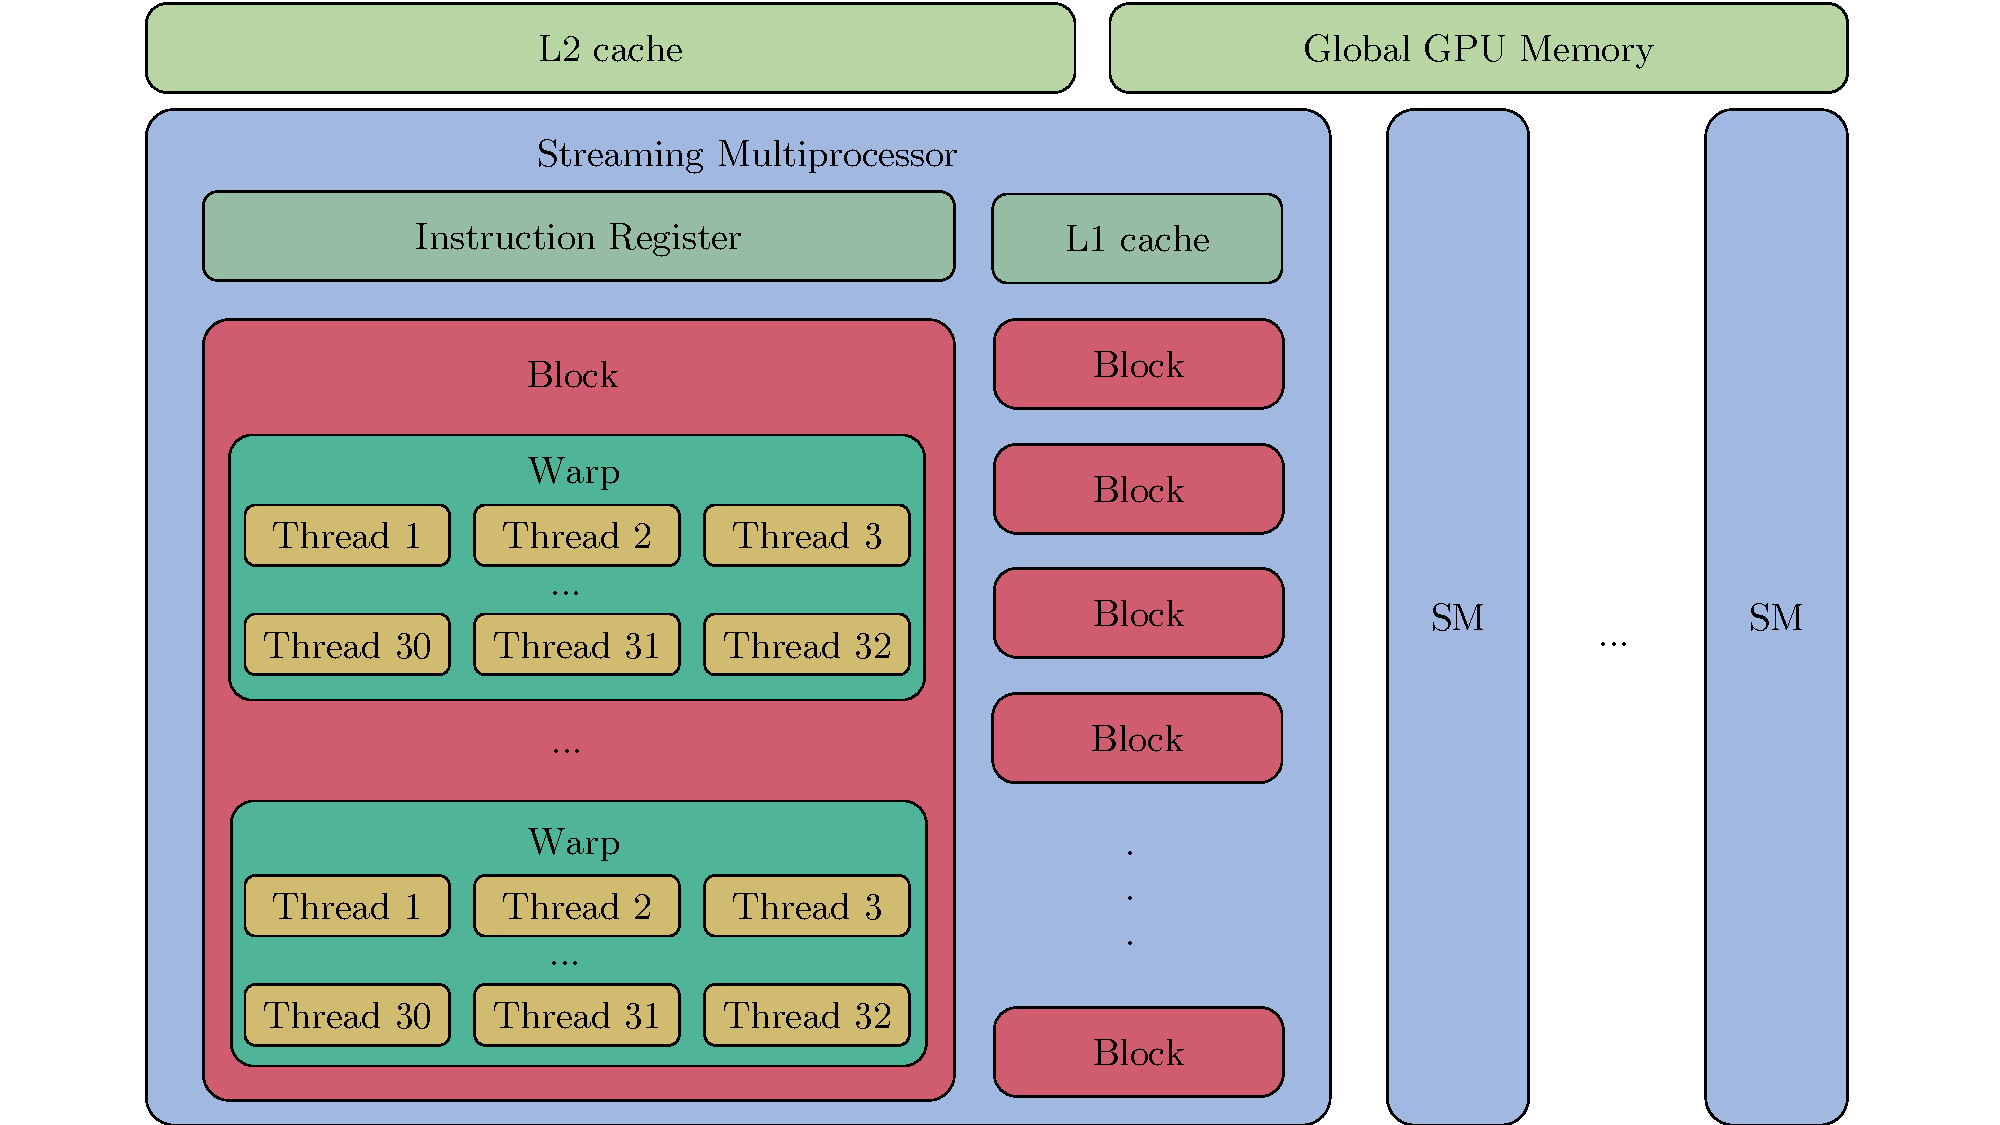
\includegraphics[width=\textwidth]{GPU_microarchitecture.pdf}
    \caption{GPU microarchitecture (figure inspiration \cite*{solvercomp})}
    \label{fig:gpu}
\end{figure}

This hierarchical structure simplifies the task of handling such a massive number of 
threads. Since only one control unit is required per warp, this leaves more space for 
packing additional threads onto the chip. Further, the large instruction register means 
that each SM can hold many instructions and dispatch them to eligible warps before 
stalling due to a data request \cite*{solvercomp}. A warp may of course need to access 
the slower L1 or L2 caches for data, but while that is happening other warps are already 
performing different operations, so that - in effect - this memory access latency is 
hidden. A potential disadvantage of this approach is that the execution time of a warp 
is limited by the slowest thread in the warp forcing others to idle. If the execution 
time between threads in a warp is large, this effect is called \emph{thread divergence}. \\

An important consideration when launching computations on the GPU (known as \emph{kernels}) 
is the block size. Since all threads in a SM must share the instruction register, 
increasing the block size (and therefore the number of threads controlled by the SM) means 
that there will necessarily be less register slots per thread. Conversely, decreasing 
block size will increase available register slots per thread, but will mean less threads 
total can be launched by the SM, since each SM has a maximal number of residing threads 
determined by the hardware. 

\begin{definition}
    \cite*{occupancy, solvercomp} We call the ratio of the number of residing threads $n$ 
    in a SM vs the theoretical maximum number of threads $N$ per SM allowed by the hardware 
    the \emph{occupancy $O$}, that is, $O = n / N$.
\end{definition}

\begin{example}
    Nvidia's Ampere architecture supports a maximum of $N = 2048$ threads per SM, each with 
    65536 register slots and maximal block count of 32. Supported block sizes range from 1 
    to 1024, and a maximum of 255 register slots per thread \cite*{ampere}. 

    \begin{itemize} 
        \item If we choose a block size of 32 to match the size of a warp, we get the 
        maximum number of residing threads $n = 32 \cdot 32 = 1024$ and our occupancy is 
        $O = n / N = 50\%$. Each thread has access to $65536 / 1024 = 64$ register slots. 
        \item If we instead choose a block size of 64, then we reach full occupancy, but 
        each thread now only has access to 32 register slots. 
    \end{itemize}

\end{example}

The precise "best" balance between occupancy and register size is highly problem dependent, 
and there are many other hardware-based factors which affect the true achievable occupancy. 
These factors iclude, but are not limited to, unbalanced workload within / across blocks, 
launching too few blocks per SM, and not launching enough calculations to saturate all 
threads in a warp \cite*{occupancy}. 
This makes optimal GPU performance not always feasible when writing generic code. However, 
Nvidia provides an official occupancy calculator API \cite*{occupancycalc} which suggests 
appropriate thread and block counts to approximately maximize occupancy while attempting 
to ensure that threads have large enough register availability. The julia package 
\jlinl{CUDA.jl} \cite*{cuda.jl} provides a wrapper for this API, accessible by calling 
\jlinl{launch_configuration(cf)} for compiled cuda kernels \jlinl{cf}.

% -------------------------------------------------------------------------------------- %

\subsection{Implementaion in GAIO.jl}

The technique for parallelization via the GPU is quite natural: one thread is responsible 
for one test point. Initially, a more involved approach was tested, though this 
was replaced by a "naive" approach, as described in \cite*{naivegpu,solvercomp}. The 
choice was made under the motto "keep it simple, stupid". \\

With the exception of Apple's "unified" desktop system-on-chip design, memory for the CPU 
and GPU are kept separate. Hence if a computation is to be launched on the GPU, the 
respective instructions and data must first be transferred from the system 
RAM via a PCIe bus to the GPU's internal memory (VRAM). Transferring data via a 
PCIe bus is much slower than transferring data within a chip (eg. from the CPU's L1/L2 
cache to instruction registers). Hence it is ideal to reduce necessary transfers and 
perform as much of a computation solely on the GPU or CPU. \\

In order to reduce transfers, a global set of test points is calculated when the 
\jlinl{SampledBoxMap} is initialized. These points are normalized to the unit cirle w.r.t. 
$|| \cdot ||_\infty$, that is, the unit cube $[-1,1]^d$. The global test points are 
transferred only once to the GPU's VRAM at initialization, and at runtime each point $p$ 
is appropriately rescaled using \jlinl{@muladd p .* r .+ c} where $r$ and $c$ are the 
box's center and radius, respectively. This way, only the information about the 
map $f$, the partition $\mathcal{P}$, and the indices of the boxes to be mapped must be 
transferred to the GPU at runtime. Each thread calculates one index for the box containing 
the thread's mapped point, and writes this index to an array. 
Across threads we loop over test points then over box indices. This way consecutive 
threads will be assigned to test points in the same box, which (using continuity of $f$) 
reduces the chance of thread divergence. Finally, the array is 
transferred to the CPU and reduced to become the image set. The implementation of the 
kernel is shown in \autoref{lst:gpu_kernel}, and the GPU accelerated \jlinl{map_boxes}
function in \autoref{lst:boxmap_gpu}. \\

As with the CPU kernel, there are some factors only in control of the user. Modern GPUs 
are primarily designed for \emph{single-precision} operations, and are correspondingly 
much less efficient using double precision arithmetic. GAIO.jl does its best to convert 
all objects such as partitions and box sets to single precision, but again \emph{
the efficient implementation of the function $f$ is solely up to the user.
}

% -------------------------------------------------------------------------------------- %
